% Title: Block diagram of Third order noise shaper in Compact Disc Players
% Author: Ramón Jaramillo
\documentclass{article}

\usepackage{tikz}
%\usepackage{textcomp}
\begin{document}



\begin{figure}[t]
\centering
% Created by tikzDevice version 0.12.3 on 2020-04-10 11:40:59
% !TEX encoding = UTF-8 Unicode
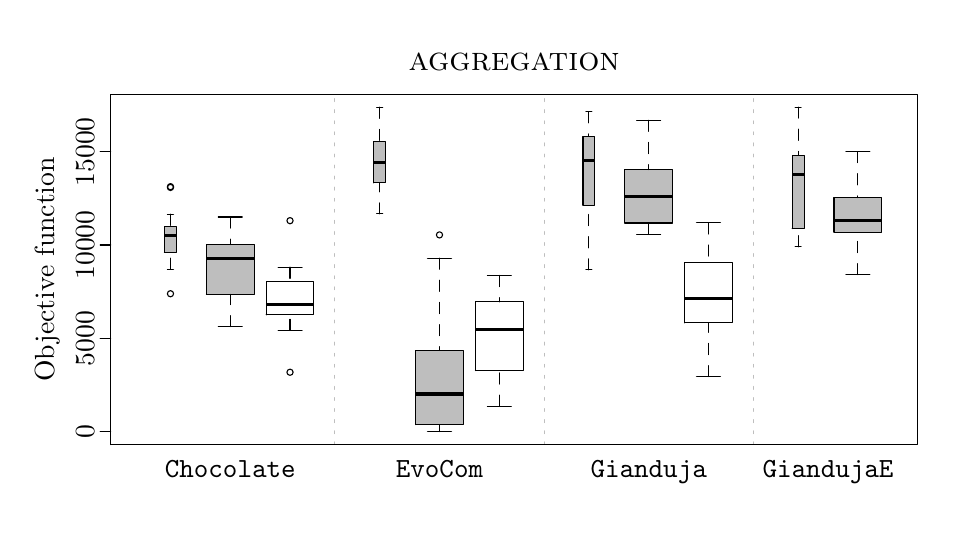
\begin{tikzpicture}[x=1pt,y=1pt]
\definecolor{fillColor}{RGB}{255,255,255}
\path[use as bounding box,fill=fillColor,fill opacity=0.00] (0,0) rectangle (325.21,180.67);
\begin{scope}
\path[clip] ( 30.00, 30.00) rectangle (321.61,156.67);
\definecolor{fillColor}{RGB}{190,190,190}

\path[fill=fillColor] ( 49.44, 99.54) --
	( 53.76, 99.54) --
	( 53.76,108.76) --
	( 49.44,108.76) --
	cycle;
\definecolor{drawColor}{RGB}{0,0,0}

\path[draw=drawColor,line width= 1.2pt,line join=round] ( 49.44,105.45) -- ( 53.76,105.45);

\path[draw=drawColor,line width= 0.4pt,dash pattern=on 4pt off 4pt ,line join=round,line cap=round] ( 51.60, 93.37) -- ( 51.60, 99.54);

\path[draw=drawColor,line width= 0.4pt,dash pattern=on 4pt off 4pt ,line join=round,line cap=round] ( 51.60,113.25) -- ( 51.60,108.76);

\path[draw=drawColor,line width= 0.4pt,line join=round,line cap=round] ( 50.52, 93.37) -- ( 52.68, 93.37);

\path[draw=drawColor,line width= 0.4pt,line join=round,line cap=round] ( 50.52,113.25) -- ( 52.68,113.25);

\path[draw=drawColor,line width= 0.4pt,line join=round,line cap=round] ( 49.44, 99.54) --
	( 53.76, 99.54) --
	( 53.76,108.76) --
	( 49.44,108.76) --
	( 49.44, 99.54);

\path[draw=drawColor,line width= 0.4pt,line join=round,line cap=round] ( 51.60, 84.53) circle (  1.12);

\path[draw=drawColor,line width= 0.4pt,line join=round,line cap=round] ( 51.60,123.22) circle (  1.12);

\path[draw=drawColor,line width= 0.4pt,line join=round,line cap=round] ( 51.60,122.94) circle (  1.12);

\path[fill=fillColor] ( 64.56, 84.30) --
	( 81.84, 84.30) --
	( 81.84,102.25) --
	( 64.56,102.25) --
	cycle;

\path[draw=drawColor,line width= 1.2pt,line join=round] ( 64.56, 97.16) -- ( 81.84, 97.16);

\path[draw=drawColor,line width= 0.4pt,dash pattern=on 4pt off 4pt ,line join=round,line cap=round] ( 73.20, 72.63) -- ( 73.20, 84.30);

\path[draw=drawColor,line width= 0.4pt,dash pattern=on 4pt off 4pt ,line join=round,line cap=round] ( 73.20,112.24) -- ( 73.20,102.25);

\path[draw=drawColor,line width= 0.4pt,line join=round,line cap=round] ( 68.88, 72.63) -- ( 77.52, 72.63);

\path[draw=drawColor,line width= 0.4pt,line join=round,line cap=round] ( 68.88,112.24) -- ( 77.52,112.24);

\path[draw=drawColor,line width= 0.4pt,line join=round,line cap=round] ( 64.56, 84.30) --
	( 81.84, 84.30) --
	( 81.84,102.25) --
	( 64.56,102.25) --
	( 64.56, 84.30);
\definecolor{fillColor}{RGB}{255,255,255}

\path[fill=fillColor] ( 86.16, 76.88) --
	(103.44, 76.88) --
	(103.44, 88.86) --
	( 86.16, 88.86) --
	cycle;

\path[draw=drawColor,line width= 1.2pt,line join=round] ( 86.16, 80.73) -- (103.44, 80.73);

\path[draw=drawColor,line width= 0.4pt,dash pattern=on 4pt off 4pt ,line join=round,line cap=round] ( 94.80, 71.28) -- ( 94.80, 76.88);

\path[draw=drawColor,line width= 0.4pt,dash pattern=on 4pt off 4pt ,line join=round,line cap=round] ( 94.80, 94.09) -- ( 94.80, 88.86);

\path[draw=drawColor,line width= 0.4pt,line join=round,line cap=round] ( 90.48, 71.28) -- ( 99.12, 71.28);

\path[draw=drawColor,line width= 0.4pt,line join=round,line cap=round] ( 90.48, 94.09) -- ( 99.12, 94.09);

\path[draw=drawColor,line width= 0.4pt,line join=round,line cap=round] ( 86.16, 76.88) --
	(103.44, 76.88) --
	(103.44, 88.86) --
	( 86.16, 88.86) --
	( 86.16, 76.88);

\path[draw=drawColor,line width= 0.4pt,line join=round,line cap=round] ( 94.80, 56.16) circle (  1.12);

\path[draw=drawColor,line width= 0.4pt,line join=round,line cap=round] ( 94.80,110.93) circle (  1.12);
\definecolor{fillColor}{RGB}{190,190,190}

\path[fill=fillColor] (125.04,124.61) --
	(129.37,124.61) --
	(129.37,139.52) --
	(125.04,139.52) --
	cycle;

\path[draw=drawColor,line width= 1.2pt,line join=round] (125.04,132.00) -- (129.37,132.00);

\path[draw=drawColor,line width= 0.4pt,dash pattern=on 4pt off 4pt ,line join=round,line cap=round] (127.20,113.38) -- (127.20,124.61);

\path[draw=drawColor,line width= 0.4pt,dash pattern=on 4pt off 4pt ,line join=round,line cap=round] (127.20,151.91) -- (127.20,139.52);

\path[draw=drawColor,line width= 0.4pt,line join=round,line cap=round] (126.12,113.38) -- (128.29,113.38);

\path[draw=drawColor,line width= 0.4pt,line join=round,line cap=round] (126.12,151.91) -- (128.29,151.91);

\path[draw=drawColor,line width= 0.4pt,line join=round,line cap=round] (125.04,124.61) --
	(129.37,124.61) --
	(129.37,139.52) --
	(125.04,139.52) --
	(125.04,124.61);

\path[fill=fillColor] (140.17, 37.23) --
	(157.45, 37.23) --
	(157.45, 64.06) --
	(140.17, 64.06) --
	cycle;

\path[draw=drawColor,line width= 1.2pt,line join=round] (140.17, 48.35) -- (157.45, 48.35);

\path[draw=drawColor,line width= 0.4pt,dash pattern=on 4pt off 4pt ,line join=round,line cap=round] (148.81, 34.69) -- (148.81, 37.23);

\path[draw=drawColor,line width= 0.4pt,dash pattern=on 4pt off 4pt ,line join=round,line cap=round] (148.81, 97.39) -- (148.81, 64.06);

\path[draw=drawColor,line width= 0.4pt,line join=round,line cap=round] (144.49, 34.69) -- (153.13, 34.69);

\path[draw=drawColor,line width= 0.4pt,line join=round,line cap=round] (144.49, 97.39) -- (153.13, 97.39);

\path[draw=drawColor,line width= 0.4pt,line join=round,line cap=round] (140.17, 37.23) --
	(157.45, 37.23) --
	(157.45, 64.06) --
	(140.17, 64.06) --
	(140.17, 37.23);

\path[draw=drawColor,line width= 0.4pt,line join=round,line cap=round] (148.81,105.79) circle (  1.12);
\definecolor{fillColor}{RGB}{255,255,255}

\path[fill=fillColor] (161.77, 56.73) --
	(179.05, 56.73) --
	(179.05, 81.60) --
	(161.77, 81.60) --
	cycle;

\path[draw=drawColor,line width= 1.2pt,line join=round] (161.77, 71.65) -- (179.05, 71.65);

\path[draw=drawColor,line width= 0.4pt,dash pattern=on 4pt off 4pt ,line join=round,line cap=round] (170.41, 43.91) -- (170.41, 56.73);

\path[draw=drawColor,line width= 0.4pt,dash pattern=on 4pt off 4pt ,line join=round,line cap=round] (170.41, 91.11) -- (170.41, 81.60);

\path[draw=drawColor,line width= 0.4pt,line join=round,line cap=round] (166.09, 43.91) -- (174.73, 43.91);

\path[draw=drawColor,line width= 0.4pt,line join=round,line cap=round] (166.09, 91.11) -- (174.73, 91.11);

\path[draw=drawColor,line width= 0.4pt,line join=round,line cap=round] (161.77, 56.73) --
	(179.05, 56.73) --
	(179.05, 81.60) --
	(161.77, 81.60) --
	(161.77, 56.73);
\definecolor{fillColor}{RGB}{190,190,190}

\path[fill=fillColor] (200.65,116.57) --
	(204.97,116.57) --
	(204.97,141.42) --
	(200.65,141.42) --
	cycle;

\path[draw=drawColor,line width= 1.2pt,line join=round] (200.65,132.60) -- (204.97,132.60);

\path[draw=drawColor,line width= 0.4pt,dash pattern=on 4pt off 4pt ,line join=round,line cap=round] (202.81, 93.15) -- (202.81,116.57);

\path[draw=drawColor,line width= 0.4pt,dash pattern=on 4pt off 4pt ,line join=round,line cap=round] (202.81,150.31) -- (202.81,141.42);

\path[draw=drawColor,line width= 0.4pt,line join=round,line cap=round] (201.73, 93.15) -- (203.89, 93.15);

\path[draw=drawColor,line width= 0.4pt,line join=round,line cap=round] (201.73,150.31) -- (203.89,150.31);

\path[draw=drawColor,line width= 0.4pt,line join=round,line cap=round] (200.65,116.57) --
	(204.97,116.57) --
	(204.97,141.42) --
	(200.65,141.42) --
	(200.65,116.57);

\path[fill=fillColor] (215.77,110.08) --
	(233.05,110.08) --
	(233.05,129.38) --
	(215.77,129.38) --
	cycle;

\path[draw=drawColor,line width= 1.2pt,line join=round] (215.77,119.54) -- (233.05,119.54);

\path[draw=drawColor,line width= 0.4pt,dash pattern=on 4pt off 4pt ,line join=round,line cap=round] (224.41,106.06) -- (224.41,110.08);

\path[draw=drawColor,line width= 0.4pt,dash pattern=on 4pt off 4pt ,line join=round,line cap=round] (224.41,147.20) -- (224.41,129.38);

\path[draw=drawColor,line width= 0.4pt,line join=round,line cap=round] (220.09,106.06) -- (228.73,106.06);

\path[draw=drawColor,line width= 0.4pt,line join=round,line cap=round] (220.09,147.20) -- (228.73,147.20);

\path[draw=drawColor,line width= 0.4pt,line join=round,line cap=round] (215.77,110.08) --
	(233.05,110.08) --
	(233.05,129.38) --
	(215.77,129.38) --
	(215.77,110.08);
\definecolor{fillColor}{RGB}{255,255,255}

\path[fill=fillColor] (237.37, 74.03) --
	(254.65, 74.03) --
	(254.65, 95.88) --
	(237.37, 95.88) --
	cycle;

\path[draw=drawColor,line width= 1.2pt,line join=round] (237.37, 82.80) -- (254.65, 82.80);

\path[draw=drawColor,line width= 0.4pt,dash pattern=on 4pt off 4pt ,line join=round,line cap=round] (246.01, 54.56) -- (246.01, 74.03);

\path[draw=drawColor,line width= 0.4pt,dash pattern=on 4pt off 4pt ,line join=round,line cap=round] (246.01,110.12) -- (246.01, 95.88);

\path[draw=drawColor,line width= 0.4pt,line join=round,line cap=round] (241.69, 54.56) -- (250.33, 54.56);

\path[draw=drawColor,line width= 0.4pt,line join=round,line cap=round] (241.69,110.12) -- (250.33,110.12);

\path[draw=drawColor,line width= 0.4pt,line join=round,line cap=round] (237.37, 74.03) --
	(254.65, 74.03) --
	(254.65, 95.88) --
	(237.37, 95.88) --
	(237.37, 74.03);
\definecolor{fillColor}{RGB}{190,190,190}

\path[fill=fillColor] (276.25,108.03) --
	(280.57,108.03) --
	(280.57,134.53) --
	(276.25,134.53) --
	cycle;

\path[draw=drawColor,line width= 1.2pt,line join=round] (276.25,127.50) -- (280.57,127.50);

\path[draw=drawColor,line width= 0.4pt,dash pattern=on 4pt off 4pt ,line join=round,line cap=round] (278.41,101.51) -- (278.41,108.03);

\path[draw=drawColor,line width= 0.4pt,dash pattern=on 4pt off 4pt ,line join=round,line cap=round] (278.41,151.98) -- (278.41,134.53);

\path[draw=drawColor,line width= 0.4pt,line join=round,line cap=round] (277.33,101.51) -- (279.49,101.51);

\path[draw=drawColor,line width= 0.4pt,line join=round,line cap=round] (277.33,151.98) -- (279.49,151.98);

\path[draw=drawColor,line width= 0.4pt,line join=round,line cap=round] (276.25,108.03) --
	(280.57,108.03) --
	(280.57,134.53) --
	(276.25,134.53) --
	(276.25,108.03);

\path[fill=fillColor] (291.37,106.81) --
	(308.65,106.81) --
	(308.65,119.24) --
	(291.37,119.24) --
	cycle;

\path[draw=drawColor,line width= 1.2pt,line join=round] (291.37,110.88) -- (308.65,110.88);

\path[draw=drawColor,line width= 0.4pt,dash pattern=on 4pt off 4pt ,line join=round,line cap=round] (300.01, 91.41) -- (300.01,106.81);

\path[draw=drawColor,line width= 0.4pt,dash pattern=on 4pt off 4pt ,line join=round,line cap=round] (300.01,135.89) -- (300.01,119.24);

\path[draw=drawColor,line width= 0.4pt,line join=round,line cap=round] (295.69, 91.41) -- (304.33, 91.41);

\path[draw=drawColor,line width= 0.4pt,line join=round,line cap=round] (295.69,135.89) -- (304.33,135.89);

\path[draw=drawColor,line width= 0.4pt,line join=round,line cap=round] (291.37,106.81) --
	(308.65,106.81) --
	(308.65,119.24) --
	(291.37,119.24) --
	(291.37,106.81);
\definecolor{drawColor}{RGB}{190,190,190}

\path[draw=drawColor,line width= 0.4pt,dash pattern=on 1pt off 3pt ,line join=round,line cap=round] (111.00, 30.00) -- (111.00,156.67);

\path[draw=drawColor,line width= 0.4pt,dash pattern=on 1pt off 3pt ,line join=round,line cap=round] (186.61, 30.00) -- (186.61,156.67);

\path[draw=drawColor,line width= 0.4pt,dash pattern=on 1pt off 3pt ,line join=round,line cap=round] (262.21, 30.00) -- (262.21,156.67);
\end{scope}
\begin{scope}
\path[clip] (  0.00,  0.00) rectangle (325.21,180.67);
\definecolor{drawColor}{RGB}{0,0,0}

\node[text=drawColor,anchor=base,inner sep=0pt, outer sep=0pt, scale=  1.00] at ( 73.20, 18.00) {\texttt{Chocolate}};

\node[text=drawColor,anchor=base,inner sep=0pt, outer sep=0pt, scale=  1.00] at (148.81, 18.00) {\texttt{EvoCom}};

\node[text=drawColor,anchor=base,inner sep=0pt, outer sep=0pt, scale=  1.00] at (224.41, 18.00) {\texttt{Gianduja}};

\node[text=drawColor,anchor=base,inner sep=0pt, outer sep=0pt, scale=  1.00] at (289.21, 18.00) {\texttt{GiandujaE}};
\end{scope}
\begin{scope}
\path[clip] (  0.00,  0.00) rectangle (325.21,180.67);
\definecolor{drawColor}{RGB}{0,0,0}

\node[text=drawColor,anchor=base,inner sep=0pt, outer sep=0pt, scale=  1.20] at (175.81,165.07) {\textsc{aggregation}};

\node[text=drawColor,rotate= 90.00,anchor=base,inner sep=0pt, outer sep=0pt, scale=  1.00] at (  9.60, 93.34) {Objective function};
\end{scope}
\begin{scope}
\path[clip] (  0.00,  0.00) rectangle (325.21,180.67);
\definecolor{drawColor}{RGB}{0,0,0}

\path[draw=drawColor,line width= 0.4pt,line join=round,line cap=round] ( 30.00, 34.69) -- ( 30.00,135.83);

\path[draw=drawColor,line width= 0.4pt,line join=round,line cap=round] ( 30.00, 34.69) -- ( 26.20, 34.69);

\path[draw=drawColor,line width= 0.4pt,line join=round,line cap=round] ( 30.00, 68.41) -- ( 26.20, 68.41);

\path[draw=drawColor,line width= 0.4pt,line join=round,line cap=round] ( 30.00,102.12) -- ( 26.20,102.12);

\path[draw=drawColor,line width= 0.4pt,line join=round,line cap=round] ( 30.00,135.83) -- ( 26.20,135.83);

\node[text=drawColor,rotate= 90.00,anchor=base,inner sep=0pt, outer sep=0pt, scale=  1.00] at ( 24.00, 34.69) {0};

\node[text=drawColor,rotate= 90.00,anchor=base,inner sep=0pt, outer sep=0pt, scale=  1.00] at ( 24.00, 68.41) {5000};

\node[text=drawColor,rotate= 90.00,anchor=base,inner sep=0pt, outer sep=0pt, scale=  1.00] at ( 24.00,102.12) {10000};

\node[text=drawColor,rotate= 90.00,anchor=base,inner sep=0pt, outer sep=0pt, scale=  1.00] at ( 24.00,135.83) {15000};

\path[draw=drawColor,line width= 0.4pt,line join=round,line cap=round] ( 30.00, 30.00) --
	(321.61, 30.00) --
	(321.61,156.67) --
	( 30.00,156.67) --
	( 30.00, 30.00);
\end{scope}
\end{tikzpicture}

\hfill
% Created by tikzDevice version 0.12 on 2019-05-07 15:15:52
% !TEX encoding = UTF-8 Unicode
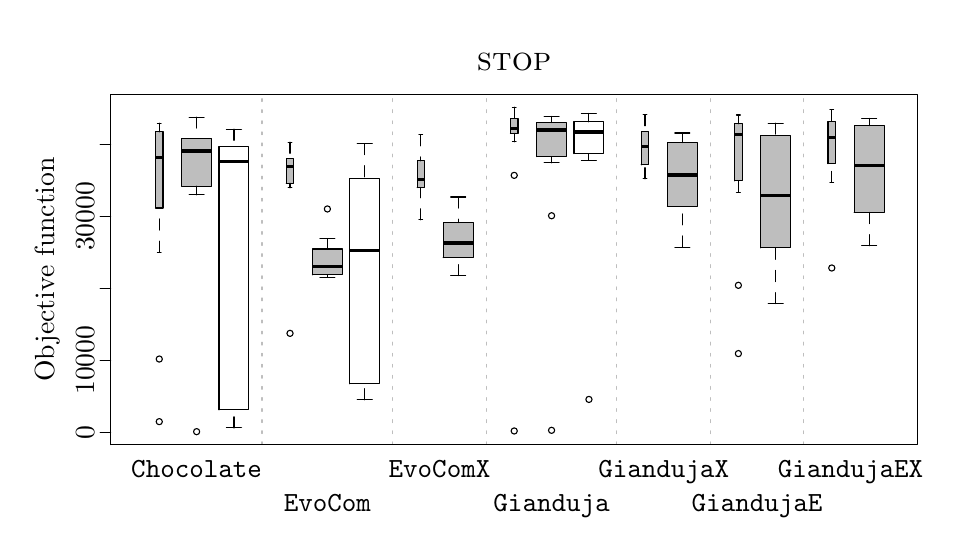
\begin{tikzpicture}[x=1pt,y=1pt]
\definecolor{fillColor}{RGB}{255,255,255}
\path[use as bounding box,fill=fillColor,fill opacity=0.00] (0,0) rectangle (325.21,180.67);
\begin{scope}
\path[clip] ( 30.00, 30.00) rectangle (321.61,156.67);
\definecolor{fillColor}{RGB}{190,190,190}

\path[fill=fillColor] ( 46.20,115.52) --
	( 48.90,115.52) --
	( 48.90,143.04) --
	( 46.20,143.04) --
	cycle;
\definecolor{drawColor}{RGB}{0,0,0}

\path[draw=drawColor,line width= 1.2pt,line join=round] ( 46.20,133.75) -- ( 48.90,133.75);

\path[draw=drawColor,line width= 0.4pt,dash pattern=on 4pt off 4pt ,line join=round,line cap=round] ( 47.55, 99.56) -- ( 47.55,115.52);

\path[draw=drawColor,line width= 0.4pt,dash pattern=on 4pt off 4pt ,line join=round,line cap=round] ( 47.55,146.15) -- ( 47.55,143.04);

\path[draw=drawColor,line width= 0.4pt,line join=round,line cap=round] ( 46.88, 99.56) -- ( 48.23, 99.56);

\path[draw=drawColor,line width= 0.4pt,line join=round,line cap=round] ( 46.88,146.15) -- ( 48.23,146.15);

\path[draw=drawColor,line width= 0.4pt,line join=round,line cap=round] ( 46.20,115.52) --
	( 48.90,115.52) --
	( 48.90,143.04) --
	( 46.20,143.04) --
	( 46.20,115.52);

\path[draw=drawColor,line width= 0.4pt,line join=round,line cap=round] ( 47.55, 60.93) circle (  1.12);

\path[draw=drawColor,line width= 0.4pt,line join=round,line cap=round] ( 47.55, 38.31) circle (  1.12);

\path[fill=fillColor] ( 55.65,123.37) --
	( 66.45,123.37) --
	( 66.45,140.78) --
	( 55.65,140.78) --
	cycle;

\path[draw=drawColor,line width= 1.2pt,line join=round] ( 55.65,136.16) -- ( 66.45,136.16);

\path[draw=drawColor,line width= 0.4pt,dash pattern=on 4pt off 4pt ,line join=round,line cap=round] ( 61.05,120.29) -- ( 61.05,123.37);

\path[draw=drawColor,line width= 0.4pt,dash pattern=on 4pt off 4pt ,line join=round,line cap=round] ( 61.05,148.35) -- ( 61.05,140.78);

\path[draw=drawColor,line width= 0.4pt,line join=round,line cap=round] ( 58.35,120.29) -- ( 63.75,120.29);

\path[draw=drawColor,line width= 0.4pt,line join=round,line cap=round] ( 58.35,148.35) -- ( 63.75,148.35);

\path[draw=drawColor,line width= 0.4pt,line join=round,line cap=round] ( 55.65,123.37) --
	( 66.45,123.37) --
	( 66.45,140.78) --
	( 55.65,140.78) --
	( 55.65,123.37);

\path[draw=drawColor,line width= 0.4pt,line join=round,line cap=round] ( 61.05, 34.69) circle (  1.12);
\definecolor{fillColor}{RGB}{255,255,255}

\path[fill=fillColor] ( 69.15, 42.59) --
	( 79.95, 42.59) --
	( 79.95,137.61) --
	( 69.15,137.61) --
	cycle;

\path[draw=drawColor,line width= 1.2pt,line join=round] ( 69.15,132.27) -- ( 79.95,132.27);

\path[draw=drawColor,line width= 0.4pt,dash pattern=on 4pt off 4pt ,line join=round,line cap=round] ( 74.55, 36.05) -- ( 74.55, 42.59);

\path[draw=drawColor,line width= 0.4pt,dash pattern=on 4pt off 4pt ,line join=round,line cap=round] ( 74.55,143.97) -- ( 74.55,137.61);

\path[draw=drawColor,line width= 0.4pt,line join=round,line cap=round] ( 71.85, 36.05) -- ( 77.25, 36.05);

\path[draw=drawColor,line width= 0.4pt,line join=round,line cap=round] ( 71.85,143.97) -- ( 77.25,143.97);

\path[draw=drawColor,line width= 0.4pt,line join=round,line cap=round] ( 69.15, 42.59) --
	( 79.95, 42.59) --
	( 79.95,137.61) --
	( 69.15,137.61) --
	( 69.15, 42.59);
\definecolor{fillColor}{RGB}{190,190,190}

\path[fill=fillColor] ( 93.45,124.44) --
	( 96.15,124.44) --
	( 96.15,133.29) --
	( 93.45,133.29) --
	cycle;

\path[draw=drawColor,line width= 1.2pt,line join=round] ( 93.45,130.43) -- ( 96.15,130.43);

\path[draw=drawColor,line width= 0.4pt,dash pattern=on 4pt off 4pt ,line join=round,line cap=round] ( 94.80,122.81) -- ( 94.80,124.44);

\path[draw=drawColor,line width= 0.4pt,dash pattern=on 4pt off 4pt ,line join=round,line cap=round] ( 94.80,139.29) -- ( 94.80,133.29);

\path[draw=drawColor,line width= 0.4pt,line join=round,line cap=round] ( 94.13,122.81) -- ( 95.48,122.81);

\path[draw=drawColor,line width= 0.4pt,line join=round,line cap=round] ( 94.13,139.29) -- ( 95.48,139.29);

\path[draw=drawColor,line width= 0.4pt,line join=round,line cap=round] ( 93.45,124.44) --
	( 96.15,124.44) --
	( 96.15,133.29) --
	( 93.45,133.29) --
	( 93.45,124.44);

\path[draw=drawColor,line width= 0.4pt,line join=round,line cap=round] ( 94.80, 70.21) circle (  1.12);

\path[fill=fillColor] (102.90, 91.38) --
	(113.70, 91.38) --
	(113.70,100.69) --
	(102.90,100.69) --
	cycle;

\path[draw=drawColor,line width= 1.2pt,line join=round] (102.90, 94.39) -- (113.70, 94.39);

\path[draw=drawColor,line width= 0.4pt,dash pattern=on 4pt off 4pt ,line join=round,line cap=round] (108.30, 90.45) -- (108.30, 91.38);

\path[draw=drawColor,line width= 0.4pt,dash pattern=on 4pt off 4pt ,line join=round,line cap=round] (108.30,104.35) -- (108.30,100.69);

\path[draw=drawColor,line width= 0.4pt,line join=round,line cap=round] (105.60, 90.45) -- (111.00, 90.45);

\path[draw=drawColor,line width= 0.4pt,line join=round,line cap=round] (105.60,104.35) -- (111.00,104.35);

\path[draw=drawColor,line width= 0.4pt,line join=round,line cap=round] (102.90, 91.38) --
	(113.70, 91.38) --
	(113.70,100.69) --
	(102.90,100.69) --
	(102.90, 91.38);

\path[draw=drawColor,line width= 0.4pt,line join=round,line cap=round] (108.30,115.16) circle (  1.12);
\definecolor{fillColor}{RGB}{255,255,255}

\path[fill=fillColor] (116.40, 52.01) --
	(127.20, 52.01) --
	(127.20,126.18) --
	(116.40,126.18) --
	cycle;

\path[draw=drawColor,line width= 1.2pt,line join=round] (116.40,100.25) -- (127.20,100.25);

\path[draw=drawColor,line width= 0.4pt,dash pattern=on 4pt off 4pt ,line join=round,line cap=round] (121.80, 46.19) -- (121.80, 52.01);

\path[draw=drawColor,line width= 0.4pt,dash pattern=on 4pt off 4pt ,line join=round,line cap=round] (121.80,138.78) -- (121.80,126.18);

\path[draw=drawColor,line width= 0.4pt,line join=round,line cap=round] (119.10, 46.19) -- (124.50, 46.19);

\path[draw=drawColor,line width= 0.4pt,line join=round,line cap=round] (119.10,138.78) -- (124.50,138.78);

\path[draw=drawColor,line width= 0.4pt,line join=round,line cap=round] (116.40, 52.01) --
	(127.20, 52.01) --
	(127.20,126.18) --
	(116.40,126.18) --
	(116.40, 52.01);
\definecolor{fillColor}{RGB}{190,190,190}

\path[fill=fillColor] (140.71,122.88) --
	(143.41,122.88) --
	(143.41,132.53) --
	(140.71,132.53) --
	cycle;

\path[draw=drawColor,line width= 1.2pt,line join=round] (140.71,125.90) -- (143.41,125.90);

\path[draw=drawColor,line width= 0.4pt,dash pattern=on 4pt off 4pt ,line join=round,line cap=round] (142.06,111.22) -- (142.06,122.88);

\path[draw=drawColor,line width= 0.4pt,dash pattern=on 4pt off 4pt ,line join=round,line cap=round] (142.06,142.00) -- (142.06,132.53);

\path[draw=drawColor,line width= 0.4pt,line join=round,line cap=round] (141.38,111.22) -- (142.73,111.22);

\path[draw=drawColor,line width= 0.4pt,line join=round,line cap=round] (141.38,142.00) -- (142.73,142.00);

\path[draw=drawColor,line width= 0.4pt,line join=round,line cap=round] (140.71,122.88) --
	(143.41,122.88) --
	(143.41,132.53) --
	(140.71,132.53) --
	(140.71,122.88);

\path[fill=fillColor] (150.16, 97.62) --
	(160.96, 97.62) --
	(160.96,110.26) --
	(150.16,110.26) --
	cycle;

\path[draw=drawColor,line width= 1.2pt,line join=round] (150.16,102.91) -- (160.96,102.91);

\path[draw=drawColor,line width= 0.4pt,dash pattern=on 4pt off 4pt ,line join=round,line cap=round] (155.56, 91.07) -- (155.56, 97.62);

\path[draw=drawColor,line width= 0.4pt,dash pattern=on 4pt off 4pt ,line join=round,line cap=round] (155.56,119.49) -- (155.56,110.26);

\path[draw=drawColor,line width= 0.4pt,line join=round,line cap=round] (152.86, 91.07) -- (158.26, 91.07);

\path[draw=drawColor,line width= 0.4pt,line join=round,line cap=round] (152.86,119.49) -- (158.26,119.49);

\path[draw=drawColor,line width= 0.4pt,line join=round,line cap=round] (150.16, 97.62) --
	(160.96, 97.62) --
	(160.96,110.26) --
	(150.16,110.26) --
	(150.16, 97.62);

\path[fill=fillColor] (174.46,142.49) --
	(177.16,142.49) --
	(177.16,148.00) --
	(174.46,148.00) --
	cycle;

\path[draw=drawColor,line width= 1.2pt,line join=round] (174.46,144.28) -- (177.16,144.28);

\path[draw=drawColor,line width= 0.4pt,dash pattern=on 4pt off 4pt ,line join=round,line cap=round] (175.81,139.41) -- (175.81,142.49);

\path[draw=drawColor,line width= 0.4pt,dash pattern=on 4pt off 4pt ,line join=round,line cap=round] (175.81,151.98) -- (175.81,148.00);

\path[draw=drawColor,line width= 0.4pt,line join=round,line cap=round] (175.13,139.41) -- (176.48,139.41);

\path[draw=drawColor,line width= 0.4pt,line join=round,line cap=round] (175.13,151.98) -- (176.48,151.98);

\path[draw=drawColor,line width= 0.4pt,line join=round,line cap=round] (174.46,142.49) --
	(177.16,142.49) --
	(177.16,148.00) --
	(174.46,148.00) --
	(174.46,142.49);

\path[draw=drawColor,line width= 0.4pt,line join=round,line cap=round] (175.81,127.30) circle (  1.12);

\path[draw=drawColor,line width= 0.4pt,line join=round,line cap=round] (175.81, 34.94) circle (  1.12);

\path[fill=fillColor] (183.91,134.06) --
	(194.71,134.06) --
	(194.71,146.38) --
	(183.91,146.38) --
	cycle;

\path[draw=drawColor,line width= 1.2pt,line join=round] (183.91,143.66) -- (194.71,143.66);

\path[draw=drawColor,line width= 0.4pt,dash pattern=on 4pt off 4pt ,line join=round,line cap=round] (189.31,131.84) -- (189.31,134.06);

\path[draw=drawColor,line width= 0.4pt,dash pattern=on 4pt off 4pt ,line join=round,line cap=round] (189.31,148.57) -- (189.31,146.38);

\path[draw=drawColor,line width= 0.4pt,line join=round,line cap=round] (186.61,131.84) -- (192.01,131.84);

\path[draw=drawColor,line width= 0.4pt,line join=round,line cap=round] (186.61,148.57) -- (192.01,148.57);

\path[draw=drawColor,line width= 0.4pt,line join=round,line cap=round] (183.91,134.06) --
	(194.71,134.06) --
	(194.71,146.38) --
	(183.91,146.38) --
	(183.91,134.06);

\path[draw=drawColor,line width= 0.4pt,line join=round,line cap=round] (189.31,112.71) circle (  1.12);

\path[draw=drawColor,line width= 0.4pt,line join=round,line cap=round] (189.31, 35.17) circle (  1.12);
\definecolor{fillColor}{RGB}{255,255,255}

\path[fill=fillColor] (197.41,135.17) --
	(208.21,135.17) --
	(208.21,146.65) --
	(197.41,146.65) --
	cycle;

\path[draw=drawColor,line width= 1.2pt,line join=round] (197.41,142.93) -- (208.21,142.93);

\path[draw=drawColor,line width= 0.4pt,dash pattern=on 4pt off 4pt ,line join=round,line cap=round] (202.81,132.77) -- (202.81,135.17);

\path[draw=drawColor,line width= 0.4pt,dash pattern=on 4pt off 4pt ,line join=round,line cap=round] (202.81,149.64) -- (202.81,146.65);

\path[draw=drawColor,line width= 0.4pt,line join=round,line cap=round] (200.11,132.77) -- (205.51,132.77);

\path[draw=drawColor,line width= 0.4pt,line join=round,line cap=round] (200.11,149.64) -- (205.51,149.64);

\path[draw=drawColor,line width= 0.4pt,line join=round,line cap=round] (197.41,135.17) --
	(208.21,135.17) --
	(208.21,146.65) --
	(197.41,146.65) --
	(197.41,135.17);

\path[draw=drawColor,line width= 0.4pt,line join=round,line cap=round] (202.81, 46.34) circle (  1.12);
\definecolor{fillColor}{RGB}{190,190,190}

\path[fill=fillColor] (221.71,131.14) --
	(224.41,131.14) --
	(224.41,143.27) --
	(221.71,143.27) --
	cycle;

\path[draw=drawColor,line width= 1.2pt,line join=round] (221.71,137.85) -- (224.41,137.85);

\path[draw=drawColor,line width= 0.4pt,dash pattern=on 4pt off 4pt ,line join=round,line cap=round] (223.06,126.08) -- (223.06,131.14);

\path[draw=drawColor,line width= 0.4pt,dash pattern=on 4pt off 4pt ,line join=round,line cap=round] (223.06,149.21) -- (223.06,143.27);

\path[draw=drawColor,line width= 0.4pt,line join=round,line cap=round] (222.38,126.08) -- (223.73,126.08);

\path[draw=drawColor,line width= 0.4pt,line join=round,line cap=round] (222.38,149.21) -- (223.73,149.21);

\path[draw=drawColor,line width= 0.4pt,line join=round,line cap=round] (221.71,131.14) --
	(224.41,131.14) --
	(224.41,143.27) --
	(221.71,143.27) --
	(221.71,131.14);

\path[fill=fillColor] (231.16,116.13) --
	(241.96,116.13) --
	(241.96,139.14) --
	(231.16,139.14) --
	cycle;

\path[draw=drawColor,line width= 1.2pt,line join=round] (231.16,127.45) -- (241.96,127.45);

\path[draw=drawColor,line width= 0.4pt,dash pattern=on 4pt off 4pt ,line join=round,line cap=round] (236.56,101.39) -- (236.56,116.13);

\path[draw=drawColor,line width= 0.4pt,dash pattern=on 4pt off 4pt ,line join=round,line cap=round] (236.56,142.59) -- (236.56,139.14);

\path[draw=drawColor,line width= 0.4pt,line join=round,line cap=round] (233.86,101.39) -- (239.26,101.39);

\path[draw=drawColor,line width= 0.4pt,line join=round,line cap=round] (233.86,142.59) -- (239.26,142.59);

\path[draw=drawColor,line width= 0.4pt,line join=round,line cap=round] (231.16,116.13) --
	(241.96,116.13) --
	(241.96,139.14) --
	(231.16,139.14) --
	(231.16,116.13);

\path[fill=fillColor] (255.46,125.29) --
	(258.16,125.29) --
	(258.16,145.96) --
	(255.46,145.96) --
	cycle;

\path[draw=drawColor,line width= 1.2pt,line join=round] (255.46,141.97) -- (258.16,141.97);

\path[draw=drawColor,line width= 0.4pt,dash pattern=on 4pt off 4pt ,line join=round,line cap=round] (256.81,121.22) -- (256.81,125.29);

\path[draw=drawColor,line width= 0.4pt,dash pattern=on 4pt off 4pt ,line join=round,line cap=round] (256.81,149.11) -- (256.81,145.96);

\path[draw=drawColor,line width= 0.4pt,line join=round,line cap=round] (256.14,121.22) -- (257.49,121.22);

\path[draw=drawColor,line width= 0.4pt,line join=round,line cap=round] (256.14,149.11) -- (257.49,149.11);

\path[draw=drawColor,line width= 0.4pt,line join=round,line cap=round] (255.46,125.29) --
	(258.16,125.29) --
	(258.16,145.96) --
	(255.46,145.96) --
	(255.46,125.29);

\path[draw=drawColor,line width= 0.4pt,line join=round,line cap=round] (256.81, 62.90) circle (  1.12);

\path[draw=drawColor,line width= 0.4pt,line join=round,line cap=round] (256.81, 87.57) circle (  1.12);

\path[fill=fillColor] (264.91,101.10) --
	(275.71,101.10) --
	(275.71,141.66) --
	(264.91,141.66) --
	cycle;

\path[draw=drawColor,line width= 1.2pt,line join=round] (264.91,120.10) -- (275.71,120.10);

\path[draw=drawColor,line width= 0.4pt,dash pattern=on 4pt off 4pt ,line join=round,line cap=round] (270.31, 80.93) -- (270.31,101.10);

\path[draw=drawColor,line width= 0.4pt,dash pattern=on 4pt off 4pt ,line join=round,line cap=round] (270.31,146.18) -- (270.31,141.66);

\path[draw=drawColor,line width= 0.4pt,line join=round,line cap=round] (267.61, 80.93) -- (273.01, 80.93);

\path[draw=drawColor,line width= 0.4pt,line join=round,line cap=round] (267.61,146.18) -- (273.01,146.18);

\path[draw=drawColor,line width= 0.4pt,line join=round,line cap=round] (264.91,101.10) --
	(275.71,101.10) --
	(275.71,141.66) --
	(264.91,141.66) --
	(264.91,101.10);

\path[fill=fillColor] (289.21,131.52) --
	(291.91,131.52) --
	(291.91,146.89) --
	(289.21,146.89) --
	cycle;

\path[draw=drawColor,line width= 1.2pt,line join=round] (289.21,141.09) -- (291.91,141.09);

\path[draw=drawColor,line width= 0.4pt,dash pattern=on 4pt off 4pt ,line join=round,line cap=round] (290.56,124.76) -- (290.56,131.52);

\path[draw=drawColor,line width= 0.4pt,dash pattern=on 4pt off 4pt ,line join=round,line cap=round] (290.56,151.00) -- (290.56,146.89);

\path[draw=drawColor,line width= 0.4pt,line join=round,line cap=round] (289.89,124.76) -- (291.24,124.76);

\path[draw=drawColor,line width= 0.4pt,line join=round,line cap=round] (289.89,151.00) -- (291.24,151.00);

\path[draw=drawColor,line width= 0.4pt,line join=round,line cap=round] (289.21,131.52) --
	(291.91,131.52) --
	(291.91,146.89) --
	(289.21,146.89) --
	(289.21,131.52);

\path[draw=drawColor,line width= 0.4pt,line join=round,line cap=round] (290.56, 93.83) circle (  1.12);

\path[fill=fillColor] (298.66,113.99) --
	(309.46,113.99) --
	(309.46,145.32) --
	(298.66,145.32) --
	cycle;

\path[draw=drawColor,line width= 1.2pt,line join=round] (298.66,130.93) -- (309.46,130.93);

\path[draw=drawColor,line width= 0.4pt,dash pattern=on 4pt off 4pt ,line join=round,line cap=round] (304.06,101.88) -- (304.06,113.99);

\path[draw=drawColor,line width= 0.4pt,dash pattern=on 4pt off 4pt ,line join=round,line cap=round] (304.06,147.87) -- (304.06,145.32);

\path[draw=drawColor,line width= 0.4pt,line join=round,line cap=round] (301.36,101.88) -- (306.76,101.88);

\path[draw=drawColor,line width= 0.4pt,line join=round,line cap=round] (301.36,147.87) -- (306.76,147.87);

\path[draw=drawColor,line width= 0.4pt,line join=round,line cap=round] (298.66,113.99) --
	(309.46,113.99) --
	(309.46,145.32) --
	(298.66,145.32) --
	(298.66,113.99);
\definecolor{drawColor}{RGB}{190,190,190}

\path[draw=drawColor,line width= 0.4pt,dash pattern=on 1pt off 3pt ,line join=round,line cap=round] ( 84.68, 30.00) -- ( 84.68,156.67);

\path[draw=drawColor,line width= 0.4pt,dash pattern=on 1pt off 3pt ,line join=round,line cap=round] (131.93, 30.00) -- (131.93,156.67);

\path[draw=drawColor,line width= 0.4pt,dash pattern=on 1pt off 3pt ,line join=round,line cap=round] (165.68, 30.00) -- (165.68,156.67);

\path[draw=drawColor,line width= 0.4pt,dash pattern=on 1pt off 3pt ,line join=round,line cap=round] (212.93, 30.00) -- (212.93,156.67);

\path[draw=drawColor,line width= 0.4pt,dash pattern=on 1pt off 3pt ,line join=round,line cap=round] (246.69, 30.00) -- (246.69,156.67);

\path[draw=drawColor,line width= 0.4pt,dash pattern=on 1pt off 3pt ,line join=round,line cap=round] (280.44, 30.00) -- (280.44,156.67);
\end{scope}
\begin{scope}
\path[clip] (  0.00,  0.00) rectangle (325.21,180.67);
\definecolor{drawColor}{RGB}{0,0,0}

\node[text=drawColor,anchor=base,inner sep=0pt, outer sep=0pt, scale=  1.00] at ( 61.05, 18.00) {\texttt{Chocolate}};

\node[text=drawColor,anchor=base,inner sep=0pt, outer sep=0pt, scale=  1.00] at (148.81, 18.00) {\texttt{EvoComX}};

\node[text=drawColor,anchor=base,inner sep=0pt, outer sep=0pt, scale=  1.00] at (229.81, 18.00) {\texttt{GiandujaX}};

\node[text=drawColor,anchor=base,inner sep=0pt, outer sep=0pt, scale=  1.00] at (297.31, 18.00) {\texttt{GiandujaEX}};

\node[text=drawColor,anchor=base,inner sep=0pt, outer sep=0pt, scale=  1.00] at (108.30,  6.00) {\texttt{EvoCom}};

\node[text=drawColor,anchor=base,inner sep=0pt, outer sep=0pt, scale=  1.00] at (189.31,  6.00) {\texttt{Gianduja}};

\node[text=drawColor,anchor=base,inner sep=0pt, outer sep=0pt, scale=  1.00] at (263.56,  6.00) {\texttt{GiandujaE}};
\end{scope}
\begin{scope}
\path[clip] (  0.00,  0.00) rectangle (325.21,180.67);
\definecolor{drawColor}{RGB}{0,0,0}

\node[text=drawColor,anchor=base,inner sep=0pt, outer sep=0pt, scale=  1.20] at (175.81,165.07) {\textsc{stop}};

\node[text=drawColor,rotate= 90.00,anchor=base,inner sep=0pt, outer sep=0pt, scale=  1.00] at (  9.60, 93.34) {Objective function};
\end{scope}
\begin{scope}
\path[clip] (  0.00,  0.00) rectangle (325.21,180.67);
\definecolor{drawColor}{RGB}{0,0,0}

\path[draw=drawColor,line width= 0.4pt,line join=round,line cap=round] ( 30.00, 34.53) -- ( 30.00,138.51);

\path[draw=drawColor,line width= 0.4pt,line join=round,line cap=round] ( 30.00, 34.53) -- ( 26.20, 34.53);

\path[draw=drawColor,line width= 0.4pt,line join=round,line cap=round] ( 30.00, 60.52) -- ( 26.20, 60.52);

\path[draw=drawColor,line width= 0.4pt,line join=round,line cap=round] ( 30.00, 86.52) -- ( 26.20, 86.52);

\path[draw=drawColor,line width= 0.4pt,line join=round,line cap=round] ( 30.00,112.51) -- ( 26.20,112.51);

\path[draw=drawColor,line width= 0.4pt,line join=round,line cap=round] ( 30.00,138.51) -- ( 26.20,138.51);

\node[text=drawColor,rotate= 90.00,anchor=base,inner sep=0pt, outer sep=0pt, scale=  1.00] at ( 24.00, 34.53) {0};

\node[text=drawColor,rotate= 90.00,anchor=base,inner sep=0pt, outer sep=0pt, scale=  1.00] at ( 24.00, 60.52) {10000};

\node[text=drawColor,rotate= 90.00,anchor=base,inner sep=0pt, outer sep=0pt, scale=  1.00] at ( 24.00,112.51) {30000};

\path[draw=drawColor,line width= 0.4pt,line join=round,line cap=round] ( 30.00, 30.00) --
	(321.61, 30.00) --
	(321.61,156.67) --
	( 30.00,156.67) --
	( 30.00, 30.00);
\end{scope}
\end{tikzpicture}

\hfill
% Created by tikzDevice version 0.12 on 2019-03-27 17:35:03
% !TEX encoding = UTF-8 Unicode
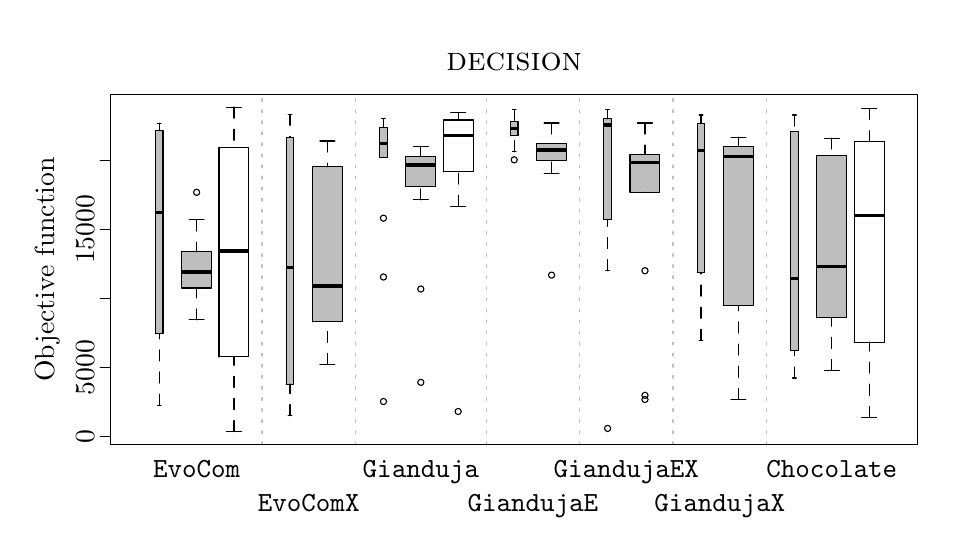
\begin{tikzpicture}[x=1pt,y=1pt]
\definecolor{fillColor}{RGB}{255,255,255}
\path[use as bounding box,fill=fillColor,fill opacity=0.00] (0,0) rectangle (325.21,180.67);
\begin{scope}
\path[clip] ( 30.00, 30.00) rectangle (321.61,156.67);
\definecolor{fillColor}{RGB}{190,190,190}

\path[fill=fillColor] ( 46.20, 70.05) --
	( 48.90, 70.05) --
	( 48.90,143.45) --
	( 46.20,143.45) --
	cycle;
\definecolor{drawColor}{RGB}{0,0,0}

\path[draw=drawColor,line width= 1.2pt,line join=round] ( 46.20,113.98) -- ( 48.90,113.98);

\path[draw=drawColor,line width= 0.4pt,dash pattern=on 4pt off 4pt ,line join=round,line cap=round] ( 47.55, 44.24) -- ( 47.55, 70.05);

\path[draw=drawColor,line width= 0.4pt,dash pattern=on 4pt off 4pt ,line join=round,line cap=round] ( 47.55,146.18) -- ( 47.55,143.45);

\path[draw=drawColor,line width= 0.4pt,line join=round,line cap=round] ( 46.88, 44.24) -- ( 48.23, 44.24);

\path[draw=drawColor,line width= 0.4pt,line join=round,line cap=round] ( 46.88,146.18) -- ( 48.23,146.18);

\path[draw=drawColor,line width= 0.4pt,line join=round,line cap=round] ( 46.20, 70.05) --
	( 48.90, 70.05) --
	( 48.90,143.45) --
	( 46.20,143.45) --
	( 46.20, 70.05);

\path[fill=fillColor] ( 55.65, 86.60) --
	( 66.45, 86.60) --
	( 66.45, 99.67) --
	( 55.65, 99.67) --
	cycle;

\path[draw=drawColor,line width= 1.2pt,line join=round] ( 55.65, 92.41) -- ( 66.45, 92.41);

\path[draw=drawColor,line width= 0.4pt,dash pattern=on 4pt off 4pt ,line join=round,line cap=round] ( 61.05, 75.08) -- ( 61.05, 86.60);

\path[draw=drawColor,line width= 0.4pt,dash pattern=on 4pt off 4pt ,line join=round,line cap=round] ( 61.05,111.20) -- ( 61.05, 99.67);

\path[draw=drawColor,line width= 0.4pt,line join=round,line cap=round] ( 58.35, 75.08) -- ( 63.75, 75.08);

\path[draw=drawColor,line width= 0.4pt,line join=round,line cap=round] ( 58.35,111.20) -- ( 63.75,111.20);

\path[draw=drawColor,line width= 0.4pt,line join=round,line cap=round] ( 55.65, 86.60) --
	( 66.45, 86.60) --
	( 66.45, 99.67) --
	( 55.65, 99.67) --
	( 55.65, 86.60);

\path[draw=drawColor,line width= 0.4pt,line join=round,line cap=round] ( 61.05,121.18) circle (  1.12);
\definecolor{fillColor}{RGB}{255,255,255}

\path[fill=fillColor] ( 69.15, 61.71) --
	( 79.95, 61.71) --
	( 79.95,137.32) --
	( 69.15,137.32) --
	cycle;

\path[draw=drawColor,line width= 1.2pt,line join=round] ( 69.15, 99.93) -- ( 79.95, 99.93);

\path[draw=drawColor,line width= 0.4pt,dash pattern=on 4pt off 4pt ,line join=round,line cap=round] ( 74.55, 34.69) -- ( 74.55, 61.71);

\path[draw=drawColor,line width= 0.4pt,dash pattern=on 4pt off 4pt ,line join=round,line cap=round] ( 74.55,151.98) -- ( 74.55,137.32);

\path[draw=drawColor,line width= 0.4pt,line join=round,line cap=round] ( 71.85, 34.69) -- ( 77.25, 34.69);

\path[draw=drawColor,line width= 0.4pt,line join=round,line cap=round] ( 71.85,151.98) -- ( 77.25,151.98);

\path[draw=drawColor,line width= 0.4pt,line join=round,line cap=round] ( 69.15, 61.71) --
	( 79.95, 61.71) --
	( 79.95,137.32) --
	( 69.15,137.32) --
	( 69.15, 61.71);
\definecolor{fillColor}{RGB}{190,190,190}

\path[fill=fillColor] ( 93.45, 51.87) --
	( 96.15, 51.87) --
	( 96.15,141.12) --
	( 93.45,141.12) --
	cycle;

\path[draw=drawColor,line width= 1.2pt,line join=round] ( 93.45, 94.06) -- ( 96.15, 94.06);

\path[draw=drawColor,line width= 0.4pt,dash pattern=on 4pt off 4pt ,line join=round,line cap=round] ( 94.80, 40.46) -- ( 94.80, 51.87);

\path[draw=drawColor,line width= 0.4pt,dash pattern=on 4pt off 4pt ,line join=round,line cap=round] ( 94.80,149.38) -- ( 94.80,141.12);

\path[draw=drawColor,line width= 0.4pt,line join=round,line cap=round] ( 94.13, 40.46) -- ( 95.48, 40.46);

\path[draw=drawColor,line width= 0.4pt,line join=round,line cap=round] ( 94.13,149.38) -- ( 95.48,149.38);

\path[draw=drawColor,line width= 0.4pt,line join=round,line cap=round] ( 93.45, 51.87) --
	( 96.15, 51.87) --
	( 96.15,141.12) --
	( 93.45,141.12) --
	( 93.45, 51.87);

\path[fill=fillColor] (102.90, 74.35) --
	(113.70, 74.35) --
	(113.70,130.35) --
	(102.90,130.35) --
	cycle;

\path[draw=drawColor,line width= 1.2pt,line join=round] (102.90, 87.33) -- (113.70, 87.33);

\path[draw=drawColor,line width= 0.4pt,dash pattern=on 4pt off 4pt ,line join=round,line cap=round] (108.30, 58.94) -- (108.30, 74.35);

\path[draw=drawColor,line width= 0.4pt,dash pattern=on 4pt off 4pt ,line join=round,line cap=round] (108.30,139.73) -- (108.30,130.35);

\path[draw=drawColor,line width= 0.4pt,line join=round,line cap=round] (105.60, 58.94) -- (111.00, 58.94);

\path[draw=drawColor,line width= 0.4pt,line join=round,line cap=round] (105.60,139.73) -- (111.00,139.73);

\path[draw=drawColor,line width= 0.4pt,line join=round,line cap=round] (102.90, 74.35) --
	(113.70, 74.35) --
	(113.70,130.35) --
	(102.90,130.35) --
	(102.90, 74.35);

\path[fill=fillColor] (127.20,133.87) --
	(129.91,133.87) --
	(129.91,144.71) --
	(127.20,144.71) --
	cycle;

\path[draw=drawColor,line width= 1.2pt,line join=round] (127.20,138.76) -- (129.91,138.76);

\path[draw=drawColor,line width= 0.4pt,dash pattern=on 4pt off 4pt ,line join=round,line cap=round] (128.56,133.87) -- (128.56,133.87);

\path[draw=drawColor,line width= 0.4pt,dash pattern=on 4pt off 4pt ,line join=round,line cap=round] (128.56,147.74) -- (128.56,144.71);

\path[draw=drawColor,line width= 0.4pt,line join=round,line cap=round] (127.88,133.87) -- (129.23,133.87);

\path[draw=drawColor,line width= 0.4pt,line join=round,line cap=round] (127.88,147.74) -- (129.23,147.74);

\path[draw=drawColor,line width= 0.4pt,line join=round,line cap=round] (127.20,133.87) --
	(129.91,133.87) --
	(129.91,144.71) --
	(127.20,144.71) --
	(127.20,133.87);

\path[draw=drawColor,line width= 0.4pt,line join=round,line cap=round] (128.56, 90.56) circle (  1.12);

\path[draw=drawColor,line width= 0.4pt,line join=round,line cap=round] (128.56, 45.58) circle (  1.12);

\path[draw=drawColor,line width= 0.4pt,line join=round,line cap=round] (128.56,111.83) circle (  1.12);

\path[fill=fillColor] (136.66,123.23) --
	(147.46,123.23) --
	(147.46,134.23) --
	(136.66,134.23) --
	cycle;

\path[draw=drawColor,line width= 1.2pt,line join=round] (136.66,131.08) -- (147.46,131.08);

\path[draw=drawColor,line width= 0.4pt,dash pattern=on 4pt off 4pt ,line join=round,line cap=round] (142.06,118.44) -- (142.06,123.23);

\path[draw=drawColor,line width= 0.4pt,dash pattern=on 4pt off 4pt ,line join=round,line cap=round] (142.06,137.80) -- (142.06,134.23);

\path[draw=drawColor,line width= 0.4pt,line join=round,line cap=round] (139.36,118.44) -- (144.76,118.44);

\path[draw=drawColor,line width= 0.4pt,line join=round,line cap=round] (139.36,137.80) -- (144.76,137.80);

\path[draw=drawColor,line width= 0.4pt,line join=round,line cap=round] (136.66,123.23) --
	(147.46,123.23) --
	(147.46,134.23) --
	(136.66,134.23) --
	(136.66,123.23);

\path[draw=drawColor,line width= 0.4pt,line join=round,line cap=round] (142.06, 86.24) circle (  1.12);

\path[draw=drawColor,line width= 0.4pt,line join=round,line cap=round] (142.06, 52.50) circle (  1.12);
\definecolor{fillColor}{RGB}{255,255,255}

\path[fill=fillColor] (150.16,128.56) --
	(160.96,128.56) --
	(160.96,147.30) --
	(150.16,147.30) --
	cycle;

\path[draw=drawColor,line width= 1.2pt,line join=round] (150.16,141.76) -- (160.96,141.76);

\path[draw=drawColor,line width= 0.4pt,dash pattern=on 4pt off 4pt ,line join=round,line cap=round] (155.56,116.14) -- (155.56,128.56);

\path[draw=drawColor,line width= 0.4pt,dash pattern=on 4pt off 4pt ,line join=round,line cap=round] (155.56,149.89) -- (155.56,147.30);

\path[draw=drawColor,line width= 0.4pt,line join=round,line cap=round] (152.86,116.14) -- (158.26,116.14);

\path[draw=drawColor,line width= 0.4pt,line join=round,line cap=round] (152.86,149.89) -- (158.26,149.89);

\path[draw=drawColor,line width= 0.4pt,line join=round,line cap=round] (150.16,128.56) --
	(160.96,128.56) --
	(160.96,147.30) --
	(150.16,147.30) --
	(150.16,128.56);

\path[draw=drawColor,line width= 0.4pt,line join=round,line cap=round] (155.56, 41.98) circle (  1.12);
\definecolor{fillColor}{RGB}{190,190,190}

\path[fill=fillColor] (174.46,141.60) --
	(177.16,141.60) --
	(177.16,146.74) --
	(174.46,146.74) --
	cycle;

\path[draw=drawColor,line width= 1.2pt,line join=round] (174.46,144.33) -- (177.16,144.33);

\path[draw=drawColor,line width= 0.4pt,dash pattern=on 4pt off 4pt ,line join=round,line cap=round] (175.81,135.84) -- (175.81,141.60);

\path[draw=drawColor,line width= 0.4pt,dash pattern=on 4pt off 4pt ,line join=round,line cap=round] (175.81,151.14) -- (175.81,146.74);

\path[draw=drawColor,line width= 0.4pt,line join=round,line cap=round] (175.13,135.84) -- (176.48,135.84);

\path[draw=drawColor,line width= 0.4pt,line join=round,line cap=round] (175.13,151.14) -- (176.48,151.14);

\path[draw=drawColor,line width= 0.4pt,line join=round,line cap=round] (174.46,141.60) --
	(177.16,141.60) --
	(177.16,146.74) --
	(174.46,146.74) --
	(174.46,141.60);

\path[draw=drawColor,line width= 0.4pt,line join=round,line cap=round] (175.81,132.91) circle (  1.12);

\path[fill=fillColor] (183.91,132.72) --
	(194.71,132.72) --
	(194.71,138.85) --
	(183.91,138.85) --
	cycle;

\path[draw=drawColor,line width= 1.2pt,line join=round] (183.91,136.42) -- (194.71,136.42);

\path[draw=drawColor,line width= 0.4pt,dash pattern=on 4pt off 4pt ,line join=round,line cap=round] (189.31,128.09) -- (189.31,132.72);

\path[draw=drawColor,line width= 0.4pt,dash pattern=on 4pt off 4pt ,line join=round,line cap=round] (189.31,146.23) -- (189.31,138.85);

\path[draw=drawColor,line width= 0.4pt,line join=round,line cap=round] (186.61,128.09) -- (192.01,128.09);

\path[draw=drawColor,line width= 0.4pt,line join=round,line cap=round] (186.61,146.23) -- (192.01,146.23);

\path[draw=drawColor,line width= 0.4pt,line join=round,line cap=round] (183.91,132.72) --
	(194.71,132.72) --
	(194.71,138.85) --
	(183.91,138.85) --
	(183.91,132.72);

\path[draw=drawColor,line width= 0.4pt,line join=round,line cap=round] (189.31, 91.25) circle (  1.12);

\path[fill=fillColor] (208.21,111.42) --
	(210.91,111.42) --
	(210.91,147.74) --
	(208.21,147.74) --
	cycle;

\path[draw=drawColor,line width= 1.2pt,line join=round] (208.21,145.50) -- (210.91,145.50);

\path[draw=drawColor,line width= 0.4pt,dash pattern=on 4pt off 4pt ,line join=round,line cap=round] (209.56, 92.84) -- (209.56,111.42);

\path[draw=drawColor,line width= 0.4pt,dash pattern=on 4pt off 4pt ,line join=round,line cap=round] (209.56,151.14) -- (209.56,147.74);

\path[draw=drawColor,line width= 0.4pt,line join=round,line cap=round] (208.88, 92.84) -- (210.23, 92.84);

\path[draw=drawColor,line width= 0.4pt,line join=round,line cap=round] (208.88,151.14) -- (210.23,151.14);

\path[draw=drawColor,line width= 0.4pt,line join=round,line cap=round] (208.21,111.42) --
	(210.91,111.42) --
	(210.91,147.74) --
	(208.21,147.74) --
	(208.21,111.42);

\path[draw=drawColor,line width= 0.4pt,line join=round,line cap=round] (209.56, 35.86) circle (  1.12);

\path[fill=fillColor] (217.66,121.22) --
	(228.46,121.22) --
	(228.46,134.81) --
	(217.66,134.81) --
	cycle;

\path[draw=drawColor,line width= 1.2pt,line join=round] (217.66,131.96) -- (228.46,131.96);

\path[draw=drawColor,line width= 0.4pt,dash pattern=on 4pt off 4pt ,line join=round,line cap=round] (223.06,121.22) -- (223.06,121.22);

\path[draw=drawColor,line width= 0.4pt,dash pattern=on 4pt off 4pt ,line join=round,line cap=round] (223.06,146.23) -- (223.06,134.81);

\path[draw=drawColor,line width= 0.4pt,line join=round,line cap=round] (220.36,121.22) -- (225.76,121.22);

\path[draw=drawColor,line width= 0.4pt,line join=round,line cap=round] (220.36,146.23) -- (225.76,146.23);

\path[draw=drawColor,line width= 0.4pt,line join=round,line cap=round] (217.66,121.22) --
	(228.46,121.22) --
	(228.46,134.81) --
	(217.66,134.81) --
	(217.66,121.22);

\path[draw=drawColor,line width= 0.4pt,line join=round,line cap=round] (223.06, 92.84) circle (  1.12);

\path[draw=drawColor,line width= 0.4pt,line join=round,line cap=round] (223.06, 46.32) circle (  1.12);

\path[draw=drawColor,line width= 0.4pt,line join=round,line cap=round] (223.06, 47.81) circle (  1.12);

\path[fill=fillColor] (241.96, 92.16) --
	(244.66, 92.16) --
	(244.66,146.12) --
	(241.96,146.12) --
	cycle;

\path[draw=drawColor,line width= 1.2pt,line join=round] (241.96,136.24) -- (244.66,136.24);

\path[draw=drawColor,line width= 0.4pt,dash pattern=on 4pt off 4pt ,line join=round,line cap=round] (243.31, 67.67) -- (243.31, 92.16);

\path[draw=drawColor,line width= 0.4pt,dash pattern=on 4pt off 4pt ,line join=round,line cap=round] (243.31,149.13) -- (243.31,146.12);

\path[draw=drawColor,line width= 0.4pt,line join=round,line cap=round] (242.64, 67.67) -- (243.99, 67.67);

\path[draw=drawColor,line width= 0.4pt,line join=round,line cap=round] (242.64,149.13) -- (243.99,149.13);

\path[draw=drawColor,line width= 0.4pt,line join=round,line cap=round] (241.96, 92.16) --
	(244.66, 92.16) --
	(244.66,146.12) --
	(241.96,146.12) --
	(241.96, 92.16);

\path[fill=fillColor] (251.41, 80.22) --
	(262.21, 80.22) --
	(262.21,137.78) --
	(251.41,137.78) --
	cycle;

\path[draw=drawColor,line width= 1.2pt,line join=round] (251.41,134.12) -- (262.21,134.12);

\path[draw=drawColor,line width= 0.4pt,dash pattern=on 4pt off 4pt ,line join=round,line cap=round] (256.81, 46.32) -- (256.81, 80.22);

\path[draw=drawColor,line width= 0.4pt,dash pattern=on 4pt off 4pt ,line join=round,line cap=round] (256.81,141.13) -- (256.81,137.78);

\path[draw=drawColor,line width= 0.4pt,line join=round,line cap=round] (254.11, 46.32) -- (259.51, 46.32);

\path[draw=drawColor,line width= 0.4pt,line join=round,line cap=round] (254.11,141.13) -- (259.51,141.13);

\path[draw=drawColor,line width= 0.4pt,line join=round,line cap=round] (251.41, 80.22) --
	(262.21, 80.22) --
	(262.21,137.78) --
	(251.41,137.78) --
	(251.41, 80.22);

\path[fill=fillColor] (275.71, 64.00) --
	(278.41, 64.00) --
	(278.41,143.20) --
	(275.71,143.20) --
	cycle;

\path[draw=drawColor,line width= 1.2pt,line join=round] (275.71, 90.01) -- (278.41, 90.01);

\path[draw=drawColor,line width= 0.4pt,dash pattern=on 4pt off 4pt ,line join=round,line cap=round] (277.06, 54.08) -- (277.06, 64.00);

\path[draw=drawColor,line width= 0.4pt,dash pattern=on 4pt off 4pt ,line join=round,line cap=round] (277.06,149.13) -- (277.06,143.20);

\path[draw=drawColor,line width= 0.4pt,line join=round,line cap=round] (276.39, 54.08) -- (277.74, 54.08);

\path[draw=drawColor,line width= 0.4pt,line join=round,line cap=round] (276.39,149.13) -- (277.74,149.13);

\path[draw=drawColor,line width= 0.4pt,line join=round,line cap=round] (275.71, 64.00) --
	(278.41, 64.00) --
	(278.41,143.20) --
	(275.71,143.20) --
	(275.71, 64.00);

\path[fill=fillColor] (285.16, 75.79) --
	(295.96, 75.79) --
	(295.96,134.63) --
	(285.16,134.63) --
	cycle;

\path[draw=drawColor,line width= 1.2pt,line join=round] (285.16, 94.49) -- (295.96, 94.49);

\path[draw=drawColor,line width= 0.4pt,dash pattern=on 4pt off 4pt ,line join=round,line cap=round] (290.56, 56.79) -- (290.56, 75.79);

\path[draw=drawColor,line width= 0.4pt,dash pattern=on 4pt off 4pt ,line join=round,line cap=round] (290.56,140.78) -- (290.56,134.63);

\path[draw=drawColor,line width= 0.4pt,line join=round,line cap=round] (287.86, 56.79) -- (293.26, 56.79);

\path[draw=drawColor,line width= 0.4pt,line join=round,line cap=round] (287.86,140.78) -- (293.26,140.78);

\path[draw=drawColor,line width= 0.4pt,line join=round,line cap=round] (285.16, 75.79) --
	(295.96, 75.79) --
	(295.96,134.63) --
	(285.16,134.63) --
	(285.16, 75.79);
\definecolor{fillColor}{RGB}{255,255,255}

\path[fill=fillColor] (298.66, 66.99) --
	(309.46, 66.99) --
	(309.46,139.48) --
	(298.66,139.48) --
	cycle;

\path[draw=drawColor,line width= 1.2pt,line join=round] (298.66,112.85) -- (309.46,112.85);

\path[draw=drawColor,line width= 0.4pt,dash pattern=on 4pt off 4pt ,line join=round,line cap=round] (304.06, 39.82) -- (304.06, 66.99);

\path[draw=drawColor,line width= 0.4pt,dash pattern=on 4pt off 4pt ,line join=round,line cap=round] (304.06,151.50) -- (304.06,139.48);

\path[draw=drawColor,line width= 0.4pt,line join=round,line cap=round] (301.36, 39.82) -- (306.76, 39.82);

\path[draw=drawColor,line width= 0.4pt,line join=round,line cap=round] (301.36,151.50) -- (306.76,151.50);

\path[draw=drawColor,line width= 0.4pt,line join=round,line cap=round] (298.66, 66.99) --
	(309.46, 66.99) --
	(309.46,139.48) --
	(298.66,139.48) --
	(298.66, 66.99);
\definecolor{drawColor}{RGB}{190,190,190}

\path[draw=drawColor,line width= 0.4pt,dash pattern=on 1pt off 3pt ,line join=round,line cap=round] ( 84.68, 30.00) -- ( 84.68,156.67);

\path[draw=drawColor,line width= 0.4pt,dash pattern=on 1pt off 3pt ,line join=round,line cap=round] (118.43, 30.00) -- (118.43,156.67);

\path[draw=drawColor,line width= 0.4pt,dash pattern=on 1pt off 3pt ,line join=round,line cap=round] (165.68, 30.00) -- (165.68,156.67);

\path[draw=drawColor,line width= 0.4pt,dash pattern=on 1pt off 3pt ,line join=round,line cap=round] (199.43, 30.00) -- (199.43,156.67);

\path[draw=drawColor,line width= 0.4pt,dash pattern=on 1pt off 3pt ,line join=round,line cap=round] (233.19, 30.00) -- (233.19,156.67);

\path[draw=drawColor,line width= 0.4pt,dash pattern=on 1pt off 3pt ,line join=round,line cap=round] (266.94, 30.00) -- (266.94,156.67);
\end{scope}
\begin{scope}
\path[clip] (  0.00,  0.00) rectangle (325.21,180.67);
\definecolor{drawColor}{RGB}{0,0,0}

\node[text=drawColor,anchor=base,inner sep=0pt, outer sep=0pt, scale=  1.00] at ( 61.05, 18.00) {\texttt{EvoCom}};

\node[text=drawColor,anchor=base,inner sep=0pt, outer sep=0pt, scale=  1.00] at (142.06, 18.00) {\texttt{Gianduja}};

\node[text=drawColor,anchor=base,inner sep=0pt, outer sep=0pt, scale=  1.00] at (216.31, 18.00) {\texttt{GiandujaEX}};

\node[text=drawColor,anchor=base,inner sep=0pt, outer sep=0pt, scale=  1.00] at (290.56, 18.00) {\texttt{Chocolate}};

\node[text=drawColor,anchor=base,inner sep=0pt, outer sep=0pt, scale=  1.00] at (101.55,  6.00) {\texttt{EvoComX}};

\node[text=drawColor,anchor=base,inner sep=0pt, outer sep=0pt, scale=  1.00] at (182.56,  6.00) {\texttt{GiandujaE}};

\node[text=drawColor,anchor=base,inner sep=0pt, outer sep=0pt, scale=  1.00] at (250.06,  6.00) {\texttt{GiandujaX}};
\end{scope}
\begin{scope}
\path[clip] (  0.00,  0.00) rectangle (325.21,180.67);
\definecolor{drawColor}{RGB}{0,0,0}

\node[text=drawColor,anchor=base,inner sep=0pt, outer sep=0pt, scale=  1.20] at (175.81,165.07) {\textsc{decision}};

\node[text=drawColor,rotate= 90.00,anchor=base,inner sep=0pt, outer sep=0pt, scale=  1.00] at (  9.60, 93.34) {Objective function};
\end{scope}
\begin{scope}
\path[clip] (  0.00,  0.00) rectangle (325.21,180.67);
\definecolor{drawColor}{RGB}{0,0,0}

\path[draw=drawColor,line width= 0.4pt,line join=round,line cap=round] ( 30.00, 32.88) -- ( 30.00,132.81);

\path[draw=drawColor,line width= 0.4pt,line join=round,line cap=round] ( 30.00, 32.88) -- ( 26.20, 32.88);

\path[draw=drawColor,line width= 0.4pt,line join=round,line cap=round] ( 30.00, 57.86) -- ( 26.20, 57.86);

\path[draw=drawColor,line width= 0.4pt,line join=round,line cap=round] ( 30.00, 82.84) -- ( 26.20, 82.84);

\path[draw=drawColor,line width= 0.4pt,line join=round,line cap=round] ( 30.00,107.82) -- ( 26.20,107.82);

\path[draw=drawColor,line width= 0.4pt,line join=round,line cap=round] ( 30.00,132.81) -- ( 26.20,132.81);

\node[text=drawColor,rotate= 90.00,anchor=base,inner sep=0pt, outer sep=0pt, scale=  1.00] at ( 24.00, 32.88) {0};

\node[text=drawColor,rotate= 90.00,anchor=base,inner sep=0pt, outer sep=0pt, scale=  1.00] at ( 24.00, 57.86) {5000};

\node[text=drawColor,rotate= 90.00,anchor=base,inner sep=0pt, outer sep=0pt, scale=  1.00] at ( 24.00,107.82) {15000};

\path[draw=drawColor,line width= 0.4pt,line join=round,line cap=round] ( 30.00, 30.00) --
	(321.61, 30.00) --
	(321.61,156.67) --
	( 30.00,156.67) --
	( 30.00, 30.00);
\end{scope}
\end{tikzpicture}

\caption{
Thick gray boxes represent the results of robot experiments;
Thick white boxes those of pseudo-reality; thin gray ones,
those of simulations.}
\label{fig:task1res}
\end{figure}

\begin{figure}[t]
\centering
% Created by tikzDevice version 0.12 on 2019-01-03 18:24:28
% !TEX encoding = UTF-8 Unicode
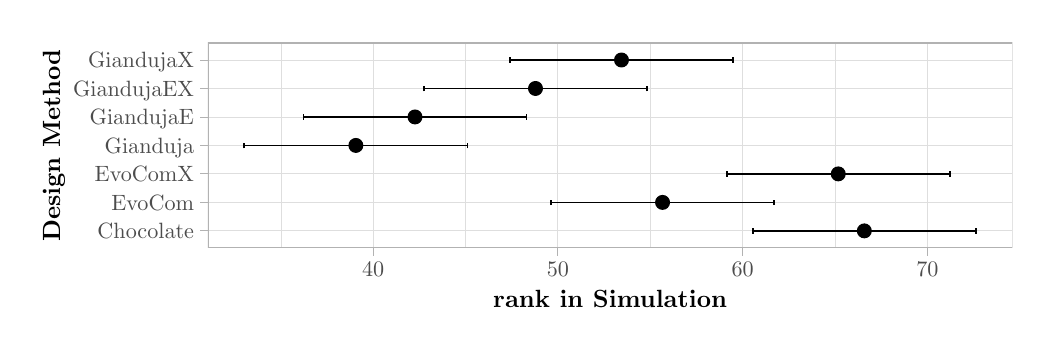
\begin{tikzpicture}[x=1pt,y=1pt]
\definecolor{fillColor}{RGB}{255,255,255}
\path[use as bounding box,fill=fillColor,fill opacity=0.00] (0,0) rectangle (361.35,108.41);
\begin{scope}
\path[clip] (  0.00,  0.00) rectangle (361.35,108.40);
\definecolor{drawColor}{RGB}{255,255,255}
\definecolor{fillColor}{RGB}{255,255,255}

\path[draw=drawColor,line width= 0.6pt,line join=round,line cap=round,fill=fillColor] (  0.00,  0.00) rectangle (361.35,108.40);
\end{scope}
\begin{scope}
\path[clip] ( 65.07, 28.81) rectangle (355.85,102.90);
\definecolor{fillColor}{RGB}{255,255,255}

\path[fill=fillColor] ( 65.07, 28.81) rectangle (355.85,102.90);
\definecolor{drawColor}{gray}{0.87}

\path[draw=drawColor,line width= 0.1pt,line join=round] ( 91.45, 28.81) --
	( 91.45,102.90);

\path[draw=drawColor,line width= 0.1pt,line join=round] (158.20, 28.81) --
	(158.20,102.90);

\path[draw=drawColor,line width= 0.1pt,line join=round] (224.96, 28.81) --
	(224.96,102.90);

\path[draw=drawColor,line width= 0.1pt,line join=round] (291.72, 28.81) --
	(291.72,102.90);

\path[draw=drawColor,line width= 0.3pt,line join=round] ( 65.07, 34.98) --
	(355.85, 34.98);

\path[draw=drawColor,line width= 0.3pt,line join=round] ( 65.07, 45.27) --
	(355.85, 45.27);

\path[draw=drawColor,line width= 0.3pt,line join=round] ( 65.07, 55.57) --
	(355.85, 55.57);

\path[draw=drawColor,line width= 0.3pt,line join=round] ( 65.07, 65.86) --
	(355.85, 65.86);

\path[draw=drawColor,line width= 0.3pt,line join=round] ( 65.07, 76.15) --
	(355.85, 76.15);

\path[draw=drawColor,line width= 0.3pt,line join=round] ( 65.07, 86.44) --
	(355.85, 86.44);

\path[draw=drawColor,line width= 0.3pt,line join=round] ( 65.07, 96.73) --
	(355.85, 96.73);

\path[draw=drawColor,line width= 0.3pt,line join=round] (124.82, 28.81) --
	(124.82,102.90);

\path[draw=drawColor,line width= 0.3pt,line join=round] (191.58, 28.81) --
	(191.58,102.90);

\path[draw=drawColor,line width= 0.3pt,line join=round] (258.34, 28.81) --
	(258.34,102.90);

\path[draw=drawColor,line width= 0.3pt,line join=round] (325.09, 28.81) --
	(325.09,102.90);
\definecolor{drawColor}{RGB}{0,0,0}
\definecolor{fillColor}{RGB}{0,0,0}

\path[draw=drawColor,line width= 0.4pt,line join=round,line cap=round,fill=fillColor] (302.32, 34.98) circle (  2.50);

\path[draw=drawColor,line width= 0.4pt,line join=round,line cap=round,fill=fillColor] (229.41, 45.27) circle (  2.50);

\path[draw=drawColor,line width= 0.4pt,line join=round,line cap=round,fill=fillColor] (292.90, 55.57) circle (  2.50);

\path[draw=drawColor,line width= 0.4pt,line join=round,line cap=round,fill=fillColor] (118.59, 65.86) circle (  2.50);

\path[draw=drawColor,line width= 0.4pt,line join=round,line cap=round,fill=fillColor] (139.96, 76.15) circle (  2.50);

\path[draw=drawColor,line width= 0.4pt,line join=round,line cap=round,fill=fillColor] (183.50, 86.44) circle (  2.50);

\path[draw=drawColor,line width= 0.4pt,line join=round,line cap=round,fill=fillColor] (214.57, 96.73) circle (  2.50);

\path[draw=drawColor,line width= 0.6pt,line join=round] (342.63, 33.95) --
	(342.63, 36.01);

\path[draw=drawColor,line width= 0.6pt,line join=round] (342.63, 34.98) --
	(262.01, 34.98);

\path[draw=drawColor,line width= 0.6pt,line join=round] (262.01, 33.95) --
	(262.01, 36.01);

\path[draw=drawColor,line width= 0.6pt,line join=round] (269.72, 44.25) --
	(269.72, 46.30);

\path[draw=drawColor,line width= 0.6pt,line join=round] (269.72, 45.27) --
	(189.10, 45.27);

\path[draw=drawColor,line width= 0.6pt,line join=round] (189.10, 44.25) --
	(189.10, 46.30);

\path[draw=drawColor,line width= 0.6pt,line join=round] (333.21, 54.54) --
	(333.21, 56.59);

\path[draw=drawColor,line width= 0.6pt,line join=round] (333.21, 55.57) --
	(252.59, 55.57);

\path[draw=drawColor,line width= 0.6pt,line join=round] (252.59, 54.54) --
	(252.59, 56.59);

\path[draw=drawColor,line width= 0.6pt,line join=round] (158.90, 64.83) --
	(158.90, 66.89);

\path[draw=drawColor,line width= 0.6pt,line join=round] (158.90, 65.86) --
	( 78.28, 65.86);

\path[draw=drawColor,line width= 0.6pt,line join=round] ( 78.28, 64.83) --
	( 78.28, 66.89);

\path[draw=drawColor,line width= 0.6pt,line join=round] (180.27, 75.12) --
	(180.27, 77.18);

\path[draw=drawColor,line width= 0.6pt,line join=round] (180.27, 76.15) --
	( 99.65, 76.15);

\path[draw=drawColor,line width= 0.6pt,line join=round] ( 99.65, 75.12) --
	( 99.65, 77.18);

\path[draw=drawColor,line width= 0.6pt,line join=round] (223.81, 85.41) --
	(223.81, 87.47);

\path[draw=drawColor,line width= 0.6pt,line join=round] (223.81, 86.44) --
	(143.19, 86.44);

\path[draw=drawColor,line width= 0.6pt,line join=round] (143.19, 85.41) --
	(143.19, 87.47);

\path[draw=drawColor,line width= 0.6pt,line join=round] (254.88, 95.70) --
	(254.88, 97.76);

\path[draw=drawColor,line width= 0.6pt,line join=round] (254.88, 96.73) --
	(174.26, 96.73);

\path[draw=drawColor,line width= 0.6pt,line join=round] (174.26, 95.70) --
	(174.26, 97.76);
\definecolor{drawColor}{gray}{0.70}

\path[draw=drawColor,line width= 0.6pt,line join=round,line cap=round] ( 65.07, 28.81) rectangle (355.85,102.90);
\end{scope}
\begin{scope}
\path[clip] (  0.00,  0.00) rectangle (361.35,108.41);
\definecolor{drawColor}{gray}{0.30}

\node[text=drawColor,anchor=base east,inner sep=0pt, outer sep=0pt, scale=  0.80] at ( 60.12, 32.23) {Chocolate};

\node[text=drawColor,anchor=base east,inner sep=0pt, outer sep=0pt, scale=  0.80] at ( 60.12, 42.52) {EvoCom};

\node[text=drawColor,anchor=base east,inner sep=0pt, outer sep=0pt, scale=  0.80] at ( 60.12, 52.81) {EvoComX};

\node[text=drawColor,anchor=base east,inner sep=0pt, outer sep=0pt, scale=  0.80] at ( 60.12, 63.10) {Gianduja};

\node[text=drawColor,anchor=base east,inner sep=0pt, outer sep=0pt, scale=  0.80] at ( 60.12, 73.39) {GiandujaE};

\node[text=drawColor,anchor=base east,inner sep=0pt, outer sep=0pt, scale=  0.80] at ( 60.12, 83.68) {GiandujaEX};

\node[text=drawColor,anchor=base east,inner sep=0pt, outer sep=0pt, scale=  0.80] at ( 60.12, 93.98) {GiandujaX};
\end{scope}
\begin{scope}
\path[clip] (  0.00,  0.00) rectangle (361.35,108.41);
\definecolor{drawColor}{gray}{0.70}

\path[draw=drawColor,line width= 0.3pt,line join=round] ( 62.32, 34.98) --
	( 65.07, 34.98);

\path[draw=drawColor,line width= 0.3pt,line join=round] ( 62.32, 45.27) --
	( 65.07, 45.27);

\path[draw=drawColor,line width= 0.3pt,line join=round] ( 62.32, 55.57) --
	( 65.07, 55.57);

\path[draw=drawColor,line width= 0.3pt,line join=round] ( 62.32, 65.86) --
	( 65.07, 65.86);

\path[draw=drawColor,line width= 0.3pt,line join=round] ( 62.32, 76.15) --
	( 65.07, 76.15);

\path[draw=drawColor,line width= 0.3pt,line join=round] ( 62.32, 86.44) --
	( 65.07, 86.44);

\path[draw=drawColor,line width= 0.3pt,line join=round] ( 62.32, 96.73) --
	( 65.07, 96.73);
\end{scope}
\begin{scope}
\path[clip] (  0.00,  0.00) rectangle (361.35,108.41);
\definecolor{drawColor}{gray}{0.70}

\path[draw=drawColor,line width= 0.3pt,line join=round] (124.82, 26.06) --
	(124.82, 28.81);

\path[draw=drawColor,line width= 0.3pt,line join=round] (191.58, 26.06) --
	(191.58, 28.81);

\path[draw=drawColor,line width= 0.3pt,line join=round] (258.34, 26.06) --
	(258.34, 28.81);

\path[draw=drawColor,line width= 0.3pt,line join=round] (325.09, 26.06) --
	(325.09, 28.81);
\end{scope}
\begin{scope}
\path[clip] (  0.00,  0.00) rectangle (361.35,108.41);
\definecolor{drawColor}{gray}{0.30}

\node[text=drawColor,anchor=base,inner sep=0pt, outer sep=0pt, scale=  0.80] at (124.82, 18.35) {40};

\node[text=drawColor,anchor=base,inner sep=0pt, outer sep=0pt, scale=  0.80] at (191.58, 18.35) {50};

\node[text=drawColor,anchor=base,inner sep=0pt, outer sep=0pt, scale=  0.80] at (258.34, 18.35) {60};

\node[text=drawColor,anchor=base,inner sep=0pt, outer sep=0pt, scale=  0.80] at (325.09, 18.35) {70};
\end{scope}
\begin{scope}
\path[clip] (  0.00,  0.00) rectangle (361.35,108.41);
\definecolor{drawColor}{RGB}{0,0,0}

\node[text=drawColor,anchor=base,inner sep=0pt, outer sep=0pt, scale=  0.90] at (210.46,  7.44) {\bfseries rank in Simulation};
\end{scope}
\begin{scope}
\path[clip] (  0.00,  0.00) rectangle (361.35,108.41);
\definecolor{drawColor}{RGB}{0,0,0}

\node[text=drawColor,rotate= 90.00,anchor=base,inner sep=0pt, outer sep=0pt, scale=  0.90] at ( 11.71, 65.86) {\bfseries Design Method};
\end{scope}
\end{tikzpicture}

\caption{Friedman test on the aggregated results of the three missions. The
  plot represents the average rank of the seven methods and their
  95\% confidence interval. }
\label{fig:friedmanSIM}
\end{figure}

\begin{figure}[t]
\centering
% Created by tikzDevice version 0.12 on 2019-03-12 12:51:42
% !TEX encoding = UTF-8 Unicode
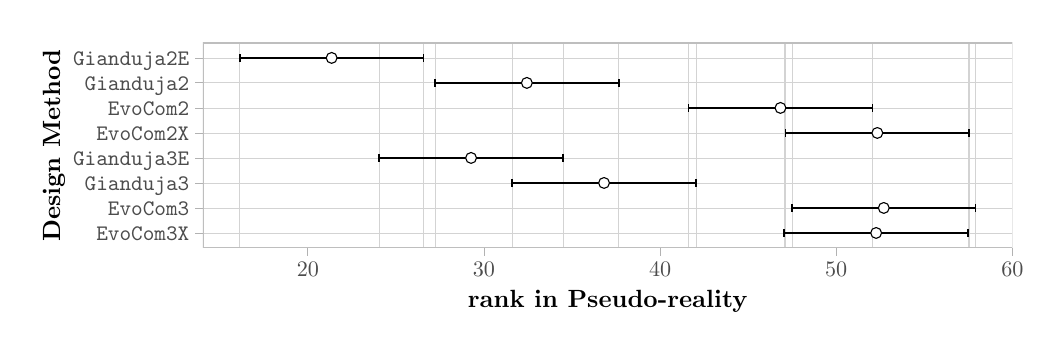
\begin{tikzpicture}[x=1pt,y=1pt]
\definecolor{fillColor}{RGB}{255,255,255}
\path[use as bounding box,fill=fillColor,fill opacity=0.00] (0,0) rectangle (361.35,108.41);
\begin{scope}
\path[clip] (  0.00,  0.00) rectangle (361.35,108.40);
\definecolor{drawColor}{RGB}{255,255,255}
\definecolor{fillColor}{RGB}{255,255,255}

\path[draw=drawColor,line width= 0.6pt,line join=round,line cap=round,fill=fillColor] (  0.00,  0.00) rectangle (361.35,108.40);
\end{scope}
\begin{scope}
\path[clip] ( 63.34, 28.81) rectangle (355.85,102.90);
\definecolor{fillColor}{RGB}{255,255,255}

\path[fill=fillColor] ( 63.34, 28.81) rectangle (355.85,102.90);
\definecolor{drawColor}{RGB}{211,211,211}

\path[draw=drawColor,line width= 0.3pt,line join=round] ( 63.34, 79.41) --
	(355.85, 79.41);

\path[draw=drawColor,line width= 0.3pt,line join=round] ( 63.34, 43.27) --
	(355.85, 43.27);

\path[draw=drawColor,line width= 0.3pt,line join=round] ( 63.34, 88.45) --
	(355.85, 88.45);

\path[draw=drawColor,line width= 0.3pt,line join=round] ( 63.34, 97.48) --
	(355.85, 97.48);

\path[draw=drawColor,line width= 0.3pt,line join=round] ( 63.34, 52.30) --
	(355.85, 52.30);

\path[draw=drawColor,line width= 0.3pt,line join=round] ( 63.34, 61.34) --
	(355.85, 61.34);

\path[draw=drawColor,line width= 0.3pt,line join=round] ( 63.34, 34.23) --
	(355.85, 34.23);

\path[draw=drawColor,line width= 0.3pt,line join=round] ( 63.34, 70.37) --
	(355.85, 70.37);

\path[draw=drawColor,line width= 0.2pt,line join=round] (305.22, 28.81) -- (305.22,102.90);

\path[draw=drawColor,line width= 0.2pt,line join=round] (340.22, 28.81) -- (340.22,102.90);

\path[draw=drawColor,line width= 0.2pt,line join=round] (213.58, 28.81) -- (213.58,102.90);

\path[draw=drawColor,line width= 0.2pt,line join=round] (143.05, 28.81) -- (143.05,102.90);

\path[draw=drawColor,line width= 0.2pt,line join=round] (342.55, 28.81) -- (342.55,102.90);

\path[draw=drawColor,line width= 0.2pt,line join=round] (339.80, 28.81) -- (339.80,102.90);

\path[draw=drawColor,line width= 0.2pt,line join=round] (241.47, 28.81) -- (241.47,102.90);

\path[draw=drawColor,line width= 0.2pt,line join=round] (193.43, 28.81) -- (193.43,102.90);

\path[draw=drawColor,line width= 0.2pt,line join=round] (238.81, 28.81) -- (238.81,102.90);

\path[draw=drawColor,line width= 0.2pt,line join=round] (273.82, 28.81) -- (273.82,102.90);

\path[draw=drawColor,line width= 0.2pt,line join=round] (147.17, 28.81) -- (147.17,102.90);

\path[draw=drawColor,line width= 0.2pt,line join=round] ( 76.64, 28.81) -- ( 76.64,102.90);

\path[draw=drawColor,line width= 0.2pt,line join=round] (276.15, 28.81) -- (276.15,102.90);

\path[draw=drawColor,line width= 0.2pt,line join=round] (273.39, 28.81) -- (273.39,102.90);

\path[draw=drawColor,line width= 0.2pt,line join=round] (175.07, 28.81) -- (175.07,102.90);

\path[draw=drawColor,line width= 0.2pt,line join=round] (127.02, 28.81) -- (127.02,102.90);
\definecolor{drawColor}{RGB}{0,0,0}

\path[draw=drawColor,line width= 0.6pt,line join=round] (305.22, 78.06) --
	(305.22, 80.77);

\path[draw=drawColor,line width= 0.6pt,line join=round] (305.22, 79.41) --
	(238.81, 79.41);

\path[draw=drawColor,line width= 0.6pt,line join=round] (238.81, 78.06) --
	(238.81, 80.77);

\path[draw=drawColor,line width= 0.6pt,line join=round] (340.22, 69.02) --
	(340.22, 71.73);

\path[draw=drawColor,line width= 0.6pt,line join=round] (340.22, 70.37) --
	(273.82, 70.37);

\path[draw=drawColor,line width= 0.6pt,line join=round] (273.82, 69.02) --
	(273.82, 71.73);

\path[draw=drawColor,line width= 0.6pt,line join=round] (213.58, 87.09) --
	(213.58, 89.80);

\path[draw=drawColor,line width= 0.6pt,line join=round] (213.58, 88.45) --
	(147.17, 88.45);

\path[draw=drawColor,line width= 0.6pt,line join=round] (147.17, 87.09) --
	(147.17, 89.80);

\path[draw=drawColor,line width= 0.6pt,line join=round] (143.05, 96.13) --
	(143.05, 98.84);

\path[draw=drawColor,line width= 0.6pt,line join=round] (143.05, 97.48) --
	( 76.64, 97.48);

\path[draw=drawColor,line width= 0.6pt,line join=round] ( 76.64, 96.13) --
	( 76.64, 98.84);

\path[draw=drawColor,line width= 0.6pt,line join=round] (342.55, 41.91) --
	(342.55, 44.62);

\path[draw=drawColor,line width= 0.6pt,line join=round] (342.55, 43.27) --
	(276.15, 43.27);

\path[draw=drawColor,line width= 0.6pt,line join=round] (276.15, 41.91) --
	(276.15, 44.62);

\path[draw=drawColor,line width= 0.6pt,line join=round] (339.80, 32.87) --
	(339.80, 35.59);

\path[draw=drawColor,line width= 0.6pt,line join=round] (339.80, 34.23) --
	(273.39, 34.23);

\path[draw=drawColor,line width= 0.6pt,line join=round] (273.39, 32.87) --
	(273.39, 35.59);

\path[draw=drawColor,line width= 0.6pt,line join=round] (241.47, 50.95) --
	(241.47, 53.66);

\path[draw=drawColor,line width= 0.6pt,line join=round] (241.47, 52.30) --
	(175.07, 52.30);

\path[draw=drawColor,line width= 0.6pt,line join=round] (175.07, 50.95) --
	(175.07, 53.66);

\path[draw=drawColor,line width= 0.6pt,line join=round] (193.43, 59.98) --
	(193.43, 62.69);

\path[draw=drawColor,line width= 0.6pt,line join=round] (193.43, 61.34) --
	(127.02, 61.34);

\path[draw=drawColor,line width= 0.6pt,line join=round] (127.02, 59.98) --
	(127.02, 62.69);

\path[draw=drawColor,line width= 0.4pt,line join=round,line cap=round,fill=fillColor] (272.02, 79.41) circle (  1.96);

\path[draw=drawColor,line width= 0.4pt,line join=round,line cap=round,fill=fillColor] (307.02, 70.37) circle (  1.96);

\path[draw=drawColor,line width= 0.4pt,line join=round,line cap=round,fill=fillColor] (180.38, 88.45) circle (  1.96);

\path[draw=drawColor,line width= 0.4pt,line join=round,line cap=round,fill=fillColor] (109.84, 97.48) circle (  1.96);

\path[draw=drawColor,line width= 0.4pt,line join=round,line cap=round,fill=fillColor] (309.35, 43.27) circle (  1.96);

\path[draw=drawColor,line width= 0.4pt,line join=round,line cap=round,fill=fillColor] (306.59, 34.23) circle (  1.96);

\path[draw=drawColor,line width= 0.4pt,line join=round,line cap=round,fill=fillColor] (208.27, 52.30) circle (  1.96);

\path[draw=drawColor,line width= 0.4pt,line join=round,line cap=round,fill=fillColor] (160.22, 61.34) circle (  1.96);
\definecolor{drawColor}{RGB}{190,190,190}

\path[draw=drawColor,line width= 0.6pt,line join=round,line cap=round] ( 63.34, 28.81) rectangle (355.85,102.90);
\end{scope}
\begin{scope}
\path[clip] (  0.00,  0.00) rectangle (361.35,108.41);
\definecolor{drawColor}{gray}{0.30}

\node[text=drawColor,anchor=base east,inner sep=0pt, outer sep=0pt, scale=  0.80] at ( 58.39, 76.66) {\texttt{EvoCom2}};

\node[text=drawColor,anchor=base east,inner sep=0pt, outer sep=0pt, scale=  0.80] at ( 58.39, 40.51) {\texttt{EvoCom3}};

\node[text=drawColor,anchor=base east,inner sep=0pt, outer sep=0pt, scale=  0.80] at ( 58.39, 85.69) {\texttt{Gianduja2}};

\node[text=drawColor,anchor=base east,inner sep=0pt, outer sep=0pt, scale=  0.80] at ( 58.39, 94.73) {\texttt{Gianduja2E}};

\node[text=drawColor,anchor=base east,inner sep=0pt, outer sep=0pt, scale=  0.80] at ( 58.39, 49.55) {\texttt{Gianduja3}};

\node[text=drawColor,anchor=base east,inner sep=0pt, outer sep=0pt, scale=  0.80] at ( 58.39, 58.58) {\texttt{Gianduja3E}};

\node[text=drawColor,anchor=base east,inner sep=0pt, outer sep=0pt, scale=  0.80] at ( 58.39, 31.48) {\texttt{EvoCom3X}};

\node[text=drawColor,anchor=base east,inner sep=0pt, outer sep=0pt, scale=  0.80] at ( 58.39, 67.62) {\texttt{EvoCom2X}};
\end{scope}
\begin{scope}
\path[clip] (  0.00,  0.00) rectangle (361.35,108.41);
\definecolor{drawColor}{gray}{0.70}

\path[draw=drawColor,line width= 0.3pt,line join=round] ( 60.59, 79.41) --
	( 63.34, 79.41);

\path[draw=drawColor,line width= 0.3pt,line join=round] ( 60.59, 43.27) --
	( 63.34, 43.27);

\path[draw=drawColor,line width= 0.3pt,line join=round] ( 60.59, 88.45) --
	( 63.34, 88.45);

\path[draw=drawColor,line width= 0.3pt,line join=round] ( 60.59, 97.48) --
	( 63.34, 97.48);

\path[draw=drawColor,line width= 0.3pt,line join=round] ( 60.59, 52.30) --
	( 63.34, 52.30);

\path[draw=drawColor,line width= 0.3pt,line join=round] ( 60.59, 61.34) --
	( 63.34, 61.34);

\path[draw=drawColor,line width= 0.3pt,line join=round] ( 60.59, 34.23) --
	( 63.34, 34.23);

\path[draw=drawColor,line width= 0.3pt,line join=round] ( 60.59, 70.37) --
	( 63.34, 70.37);
\end{scope}
\begin{scope}
\path[clip] (  0.00,  0.00) rectangle (361.35,108.41);
\definecolor{drawColor}{gray}{0.70}

\path[draw=drawColor,line width= 0.3pt,line join=round] (101.25, 26.06) --
	(101.25, 28.81);

\path[draw=drawColor,line width= 0.3pt,line join=round] (164.89, 26.06) --
	(164.89, 28.81);

\path[draw=drawColor,line width= 0.3pt,line join=round] (228.53, 26.06) --
	(228.53, 28.81);

\path[draw=drawColor,line width= 0.3pt,line join=round] (292.17, 26.06) --
	(292.17, 28.81);

\path[draw=drawColor,line width= 0.3pt,line join=round] (355.81, 26.06) --
	(355.81, 28.81);
\end{scope}
\begin{scope}
\path[clip] (  0.00,  0.00) rectangle (361.35,108.41);
\definecolor{drawColor}{gray}{0.30}

\node[text=drawColor,anchor=base,inner sep=0pt, outer sep=0pt, scale=  0.80] at (101.25, 18.35) {20};

\node[text=drawColor,anchor=base,inner sep=0pt, outer sep=0pt, scale=  0.80] at (164.89, 18.35) {30};

\node[text=drawColor,anchor=base,inner sep=0pt, outer sep=0pt, scale=  0.80] at (228.53, 18.35) {40};

\node[text=drawColor,anchor=base,inner sep=0pt, outer sep=0pt, scale=  0.80] at (292.17, 18.35) {50};

\node[text=drawColor,anchor=base,inner sep=0pt, outer sep=0pt, scale=  0.80] at (355.81, 18.35) {60};
\end{scope}
\begin{scope}
\path[clip] (  0.00,  0.00) rectangle (361.35,108.41);
\definecolor{drawColor}{RGB}{0,0,0}

\node[text=drawColor,anchor=base,inner sep=0pt, outer sep=0pt, scale=  0.90] at (209.60,  7.44) {\bfseries rank in Pseudo-reality};
\end{scope}
\begin{scope}
\path[clip] (  0.00,  0.00) rectangle (361.35,108.41);
\definecolor{drawColor}{RGB}{0,0,0}

\node[text=drawColor,rotate= 90.00,anchor=base,inner sep=0pt, outer sep=0pt, scale=  0.90] at ( 11.71, 65.86) {\bfseries Design Method};
\end{scope}
\end{tikzpicture}

\caption{Friedman test on the aggregated results of the three missions. The
  plot represents the average rank of the seven methods and their
  95\% confidence interval. }
\label{fig:friedmanPR}
\end{figure}


\end{document}
